% Copyright 2004 by Till Tantau <tantau@users.sourceforge.net>.
%
% In principle, this file can be redistributed and/or modified under
% the terms of the GNU Public License, version 2.
%
% However, this file is supposed to be a template to be modified
% for your own needs. For this reason, if you use this file as a
% template and not specifically distribute it as part of a another
% package/program, I grant the extra permission to freely copy and
% modify this file as you see fit and even to delete this copyright
% notice. 

\documentclass{beamer}

% There are many different themes available for Beamer. A comprehensive
% list with examples is given here:
% http://deic.uab.es/~iblanes/beamer_gallery/index_by_theme.html
% You can uncomment the themes below if you would like to use a different
% one:
%\usetheme{AnnArbor}
%\usetheme{Antibes}
%\usetheme{Bergen}
%\usetheme{Berkeley}
%\usetheme{Berlin}
%\usetheme{Boadilla}
%\usetheme{boxes}
%\usetheme{CambridgeUS}
%\usetheme{Copenhagen}
%\usetheme{Darmstadt}
%\usetheme{default}
%\usetheme{Frankfurt}
%\usetheme{Goettingen}
%\usetheme{Hannover}
%\usetheme{Ilmenau}
%\usetheme{JuanLesPins}
%\usetheme{Luebeck}
\usetheme{Madrid}
%\usetheme{Malmoe}
%\usetheme{Marburg}
%\usetheme{Montpellier}
%\usetheme{PaloAlto}
%\usetheme{Pittsburgh}
%\usetheme{Rochester}
%\usetheme{Singapore}
%\usetheme{Szeged}
%\usetheme{Warsaw}
\usepackage[brazil]{babel}
\usepackage[utf8]{inputenc}
\usepackage{graphicx}

\title{Sistemas Operacionais em Assembly}
\subtitle{Uma abordagem "top-bottom" com foco prático}

\author{
  Alcides Augusto
  \and 
  Paulo Raimundo
}

\institute[Universidade Federal da Bahia] {
  Colegiado de Engenharia da Computação\\
  Universidade Federal da Bahia
}


\date{MATA49 - Prog Software Básico, 2019-1}

% If you have a file called "university-logo-filename.xxx", where xxx
% is a graphic format that can be processed by latex or pdflatex,
% resp., then you can add a logo as follows:
% \pgfdeclareimage[height=0.5cm]{university-logo}{university-logo-filename}
% \logo{
%   \pgfuseimage{figuras/brasao_ufba}
% }

% Delete this, if you do not want the table of contents to pop up at
% the beginning of each subsection:
%\AtBeginSubsection[]
%{
%  \begin{frame}<beamer>{Roteiro}
%    \tableofcontents[currentsection,currentsubsection]
%  \end{frame}
%}
% Define o caminho das figuras
\graphicspath{{figuras/}}

\begin{document}

  \begin{frame}
    \titlepage
    \begin{figure}[!htb]
      \centering
      
\includegraphics[scale=0.15]{brasao_ufba}
      \label{brasaoUFBA}
    \end{figure}
  \end{frame}

  \begin{frame}{Roteiro}
    \tableofcontents
  \end{frame}

  \section{Introdução}

    \subsection{Hardware}

      \begin{frame}{Introdução}{Hardware}
        O que é um Sistema Computacional?
      \end{frame}

      \begin{frame}{Introdução}{Hardware}
        O que é um Sistema Computacional?
        \begin{itemize}
          \item Hardware
          \item Software
        \end{itemize}
      \end{frame}


      \begin{frame}{Introdução}{Hardware}
        O que é o Hardware?
      \end{frame}

      \begin{frame}{Introdução}{Hardware}
        Tudo bem\dots Todo mundo aqui já sabe\dots Dispensa comentários\dots
      \end{frame}

      \begin{frame}{Introdução}{Hardware}
        Mas permita-nos apenas destacar:
        \begin{itemize}
          \item O Hardware é máquina física\dots
        \end{itemize}
      \end{frame}

      \begin{frame}{Introdução}{Hardware}
        Permita-nos apenas destacar:
        \begin{itemize}
          \item O Hardware é máquina física que serve para\dots   
        \end{itemize}
      \end{frame}

      \begin{frame}{Introdução}{Hardware}
        Permita-nos apenas destacar:
        \begin{itemize}
          \item O Hardware é máquina física que serve para 
          \item Fazer OPERAÇÕES ALGORÍTMICAS
        \end{itemize}
      \end{frame}

      \begin{frame}{Introdução}{Hardware}
        Permita-nos apenas destacar:
        \begin{itemize}
          \item O Hardware é máquina física que serve para 
          \item Fazer OPERAÇÕES ALGORÍTMICAS
          \item Mas para que fazer tantas OPERAÇÕES ALGORÍTMICAS???
        \end{itemize}
      \end{frame}


    \subsection{Software}

      \begin{frame}{Introdução}{Software}
        \begin{itemize}
          \item Funcionalidades que o computador é capaz de promover
          \end{itemize}
      \end{frame}

      \begin{frame}{Introdução}{Software}
        \begin{itemize}
          \item Funcionalidades que o computador é capaz de promover
          \item Através de seus programas
          \end{itemize}
      \end{frame}

      \begin{frame}{Introdução}{Software}
        \begin{itemize}
          \item Funcionalidades que o computador é capaz de promover
          \item Através de seus programas
          \item Essas funcionalidades são a abstração de programas
          \end{itemize}
      \end{frame}

      \begin{frame}{Introdução}{Software}
        \begin{itemize}
          \item Funcionalidades que o computador é capaz de promover
          \item Através de seus programas
          \item Essas funcionalidades são a abstração de programas
            \begin{itemize}
              \item são o conjunto de instruções algorítmicas
            \end{itemize}
          \end{itemize}
      \end{frame}

      \begin{frame}{Introdução}{Software}
        \begin{itemize}
          \item Funcionalidades que o computador é capaz de promover
          \item Através de seus programas
          \item Essas funcionalidades são a abstração de programas
            \begin{itemize}
              \item são o conjunto de instruções algorítmicas 
              \item são geradas através das linguagens de programação.
            \end{itemize}
          \end{itemize}
      \end{frame}

    \subsection{Hard vs Software}

      \begin{frame}{Introdução}{Hard vs Software}
        \begin{itemize}
          \item O relacionamento entre Hardware e Software é "sensível"\dots
            \begin{itemize}
              \item Correspondência do tipo um-para-um?
                \begin{itemize}
                  \item instruções da linguagem de programação 
                  \item instruções binárias do hardware
                \end{itemize}
              \item Tradução adequada de instruções
            \end{itemize}
        \end{itemize}
      \end{frame}

      \begin{frame}{Introdução}{Hard vs Software}
        \begin{itemize}
          \item O relacionamento entre Hardware e Software é "sensível"\dots
            \begin{itemize}
              \item Há vários tipos de processadores!
            \end{itemize}
        \end{itemize}
      \end{frame}


      \begin{frame}{Introdução}{Hard vs Software}
        \begin{itemize}
          \item O relacionamento entre Hardware e Software é "sensível"\dots
            \begin{itemize}
              \item Há vários tipos de processadores!
              \item Portabilidade?!
            \end{itemize}
        \end{itemize}
      \end{frame}

      \begin{frame}{Introdução}{Hard vs Software}
        \begin{itemize}
          \item O relacionamento entre Hardware e Software é "sensível"\dots
            \begin{itemize}
              \item Há vários tipos de processadores!
              \item Portabilidade?!
              \item Segurança de dados?!
            \end{itemize}
        \end{itemize}
      \end{frame}

      \begin{frame}{Introdução}{Hard vs Software}
        \begin{itemize}
          \item O relacionamento entre Hardware e Software é "sensível"\dots
            \begin{itemize}
              \item Há vários tipos de processadores!
              \item Portabilidade?!
              \item Segurança de dados?!
              \item Gestão de recursos computacionais?!
            \end{itemize}
        \end{itemize}
      \end{frame}

      \begin{frame}{Introdução}{Hard vs Software}
        E agora o que fazer?
      \end{frame}

      \begin{frame}{Introdução}{Hard vs Software}
        Crie um \emph{Sistema Operacional!}
      \end{frame}

      \begin{frame}{Introdução}{Hard vs Software}
        Crie um \emph{Sistema Operacional!}\\
        "Solução do lado do Software"
      \end{frame}

  \section{SOs: fundamentos}
    \subsection{Objetivos de um SO}

      \begin{frame}{SOs: fundamentos}{Objetivos de um SO}
        \begin{itemize}
        \item Abstração
        \item Gerência
        \end{itemize}
      \end{frame}

      \begin{frame}{SOs: fundamentos}{Objetivos de um SO}
        \begin{figure}[!htb]
          \centering
          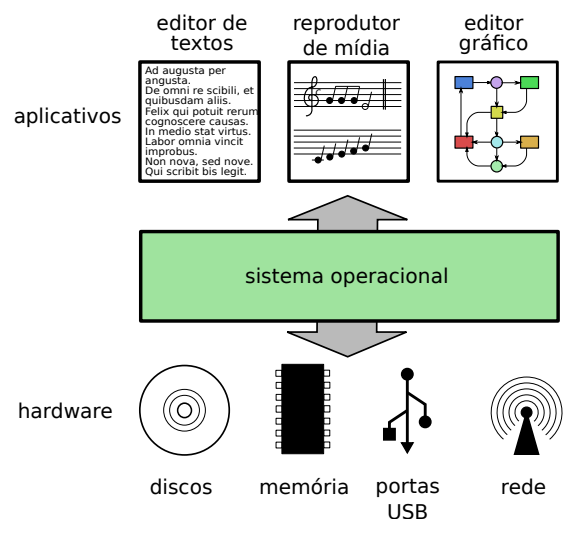
\includegraphics[width=200pt, keepaspectratio=true]{figuras/fundamentos/SOComoUmaInterface.png}
          \caption{(MAZIERO, 2019)}
          \label{SOComoUmaInterface}
        \end{figure}
      \end{frame}

    \subsection{Elementos de um SO}

      \begin{frame}{SOs: fundamentos}{Elementos de um SO}
        \begin{itemize}
        \item Programas utilitários
        \item Drivers
        \item Código de inicialização (boot code)
        \item Núcleo (kernel)
        \end{itemize}
      \end{frame}

      \subsubsection{Programas Utilitários}
      
        \begin{frame}{SOs: fundamentos}{Elementos de um SO}{\bfseries{Programas Utilitários}}
          Podem haver várias funcionalidades, exemplo:
          \begin{itemize}
            \item Terminal
            \item Manipulador de arquivos 
            \item Gerência de telas 
            \item Configurações de dispositivos
            \item Formatação de discos e mídias 
            \item Interface gráfica \\Augusto (2016) traz uma série de interfaces gráficas da família Linux \\Vejamos\dots
          \end{itemize}
        \end{frame}

        \begin{frame}{SOs: fundamentos}{Elementos de um SO}{\bfseries{Programas utilitários}}
          \begin{figure}[!htb]
            \centering
            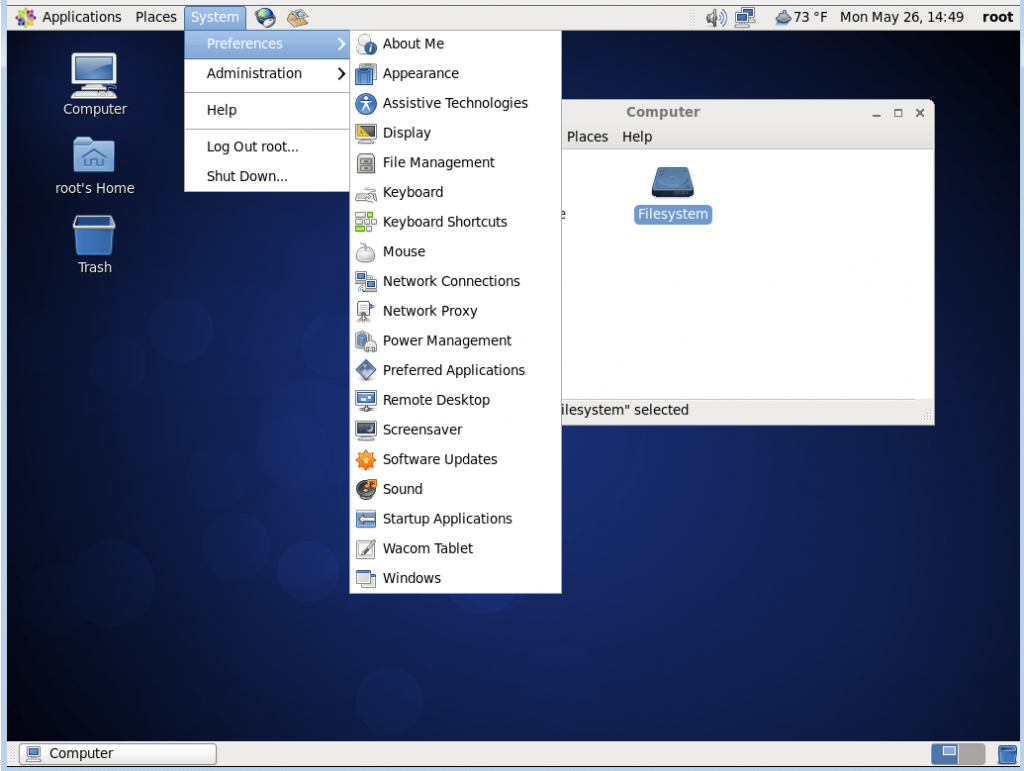
\includegraphics[width=200pt, keepaspectratio=true]{interfacesLinux/gnome_centos_6_gui_namhuy-1024x771.png}
            \caption{CentOS6 (Augusto, 2016)}
            \label{gnome_centos_6_gui_namhuy}
          \end{figure}
        \end{frame}

        \begin{frame}{SOs: fundamentos}{Elementos de um SO}{\bfseries{Programas utilitários}}
          \begin{figure}[!htb]
            \centering
            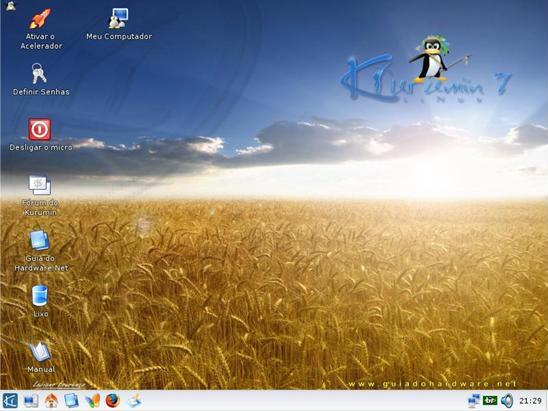
\includegraphics[width=200pt, keepaspectratio=true]{interfacesLinux/imagem-kurumin-7.jpg}
            \caption{Kurumin, (Augusto, 2016)}
            \label{imagem-kurumin-7}
          \end{figure}
        \end{frame}

        \begin{frame}{SOs: fundamentos}{Elementos de um SO}{\bfseries{Programas utilitários}}
          \begin{figure}[!htb]
            \centering
            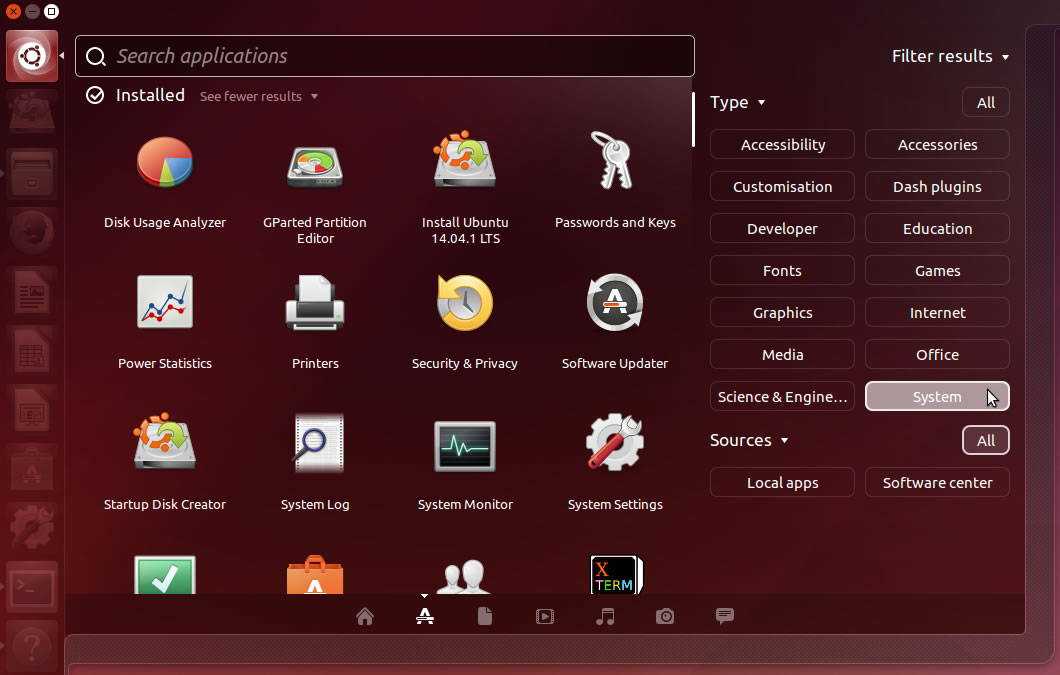
\includegraphics[width=200pt, keepaspectratio=true]{interfacesLinux/unity.jpg}
            \caption{Unity, (Augusto, 2016)}
            \label{unity}
          \end{figure}
        \end{frame}

        \begin{frame}{SOs: fundamentos}{Elementos de um SO}{\bfseries{Programas utilitários}}
          \begin{figure}[!htb]
            \centering
            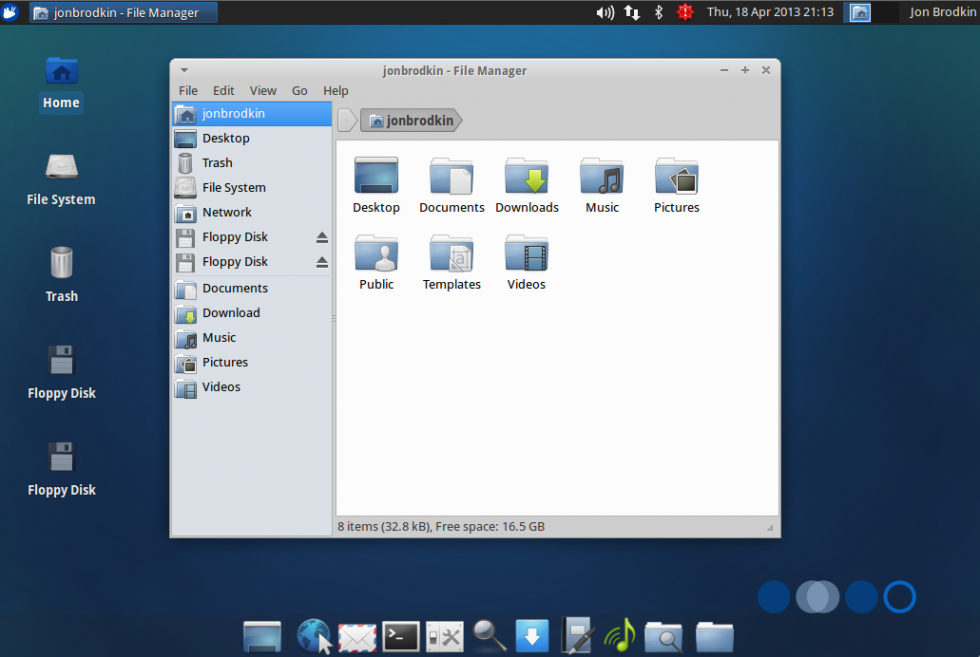
\includegraphics[width=200pt, keepaspectratio=true]{interfacesLinux/xubuntu.png}
            \caption{Xubuntu, (Augusto, 2016)}
            \label{xubuntu}
          \end{figure}
        \end{frame}


      \subsubsection{Drivers}

        \begin{frame}{SOs: fundamentos}{Elementos de um SO}{\bfseries{Drivers}}
          \newline Podem haver várias funcionalidades, exemplo:
          \begin{itemize}
            \item Módulos de códigos específicos a um dispositivo: sata, usb, vídeo\dots
            \item Comumente disponibilizado pelo fabricante do dispositivo 
            \item Funciona com se fosse um acoplamento ao SO, para que reconheça o Hardware
          \end{itemize}
        \end{frame}

      \subsubsection{Código de inicialização}
        
        \begin{frame}{SOs: fundamentos}{Elementos de um SO}{\bfseries{Código de inicialização}}
          \begin{itemize}
            \item Preparação dos dispositivos instalados
            \item Carregamento do núcleo do SO na memória RAM
            \item O bootloader:
            \begin{itemize}
              \item É a inicialização propriamente dita
              \item Tem um tamanho específicos: 512kB
              \item Tem uma assinatura convencionada (últimos 16bits)          
            \end{itemize} 
          \end{itemize}
        \end{frame}

        \begin{frame}{SOs: fundamentos}{Elementos de um SO}{\bfseries{Código de inicialização}}
          \begin{figure}[!htb]
            \centering
            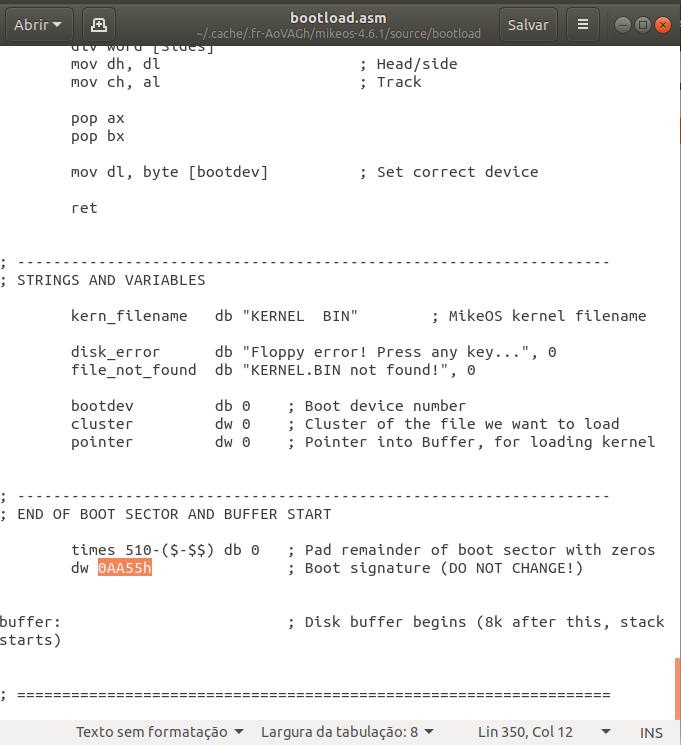
\includegraphics[width=200pt, keepaspectratio=true]{MikeOS/bootLoaderMikeOS_asm.png}
            \caption{Bootloader do MikeOS. Repare a assinatura e os bits de preenchimento. (MIKEOS, 2019)}
            \label{bootLoaderMikeOS_asm}
          \end{figure}
        \end{frame}

        \begin{frame}{SOs: fundamentos}{Elementos de um SO}{\bfseries{Código de inicialização}}
          \begin{figure}[!htb]
            \centering
            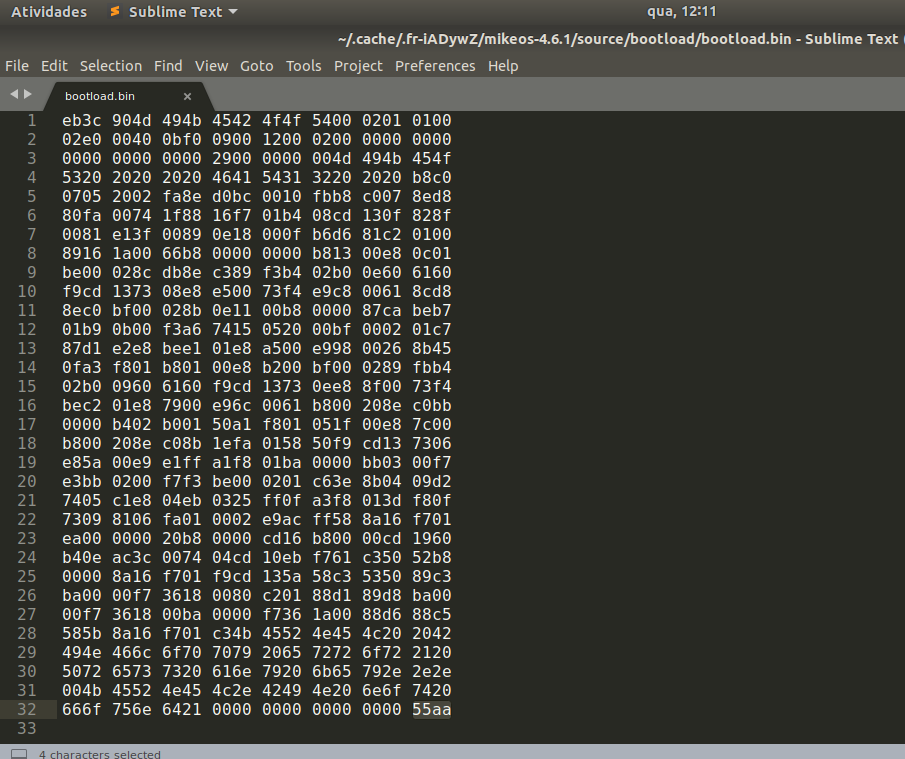
\includegraphics[width=200pt, keepaspectratio=true]{MikeOS/bootloaderMikeOS_bin.png}
            \caption{Código compilado do Bootloader do MikeOS em hexadecimal. Repare a assinatura destacada nos quatro últimos bits e seus bits anteriores preenchidos com zero. (MIKEOS, 2019)}
            \label{bootloaderMikeOS_bin}
          \end{figure}
        \end{frame}
      \subsubsection{Núcleo (kernel)}
        
        \begin{frame}{SOs: fundamentos}{Elementos de um SO}{\bfseries{Núcleo (kernel)}}
          \begin{itemize}
            \item "Coração" do sistema operacional
            \item Gerência dos recursos de hardware
            \item Implementação de diversas abstrações para:
            \begin{itemize}
              \item Aplicativos
              \item Utilitários do sistema
            \end{itemize} 
          \end{itemize}
        \end{frame}

        \begin{frame}{SOs: fundamentos}{Elementos de um SO}{\bfseries{Núcleo (kernel)}}
          \begin{itemize}
            \item O kenel Linux é um dos mais famosos e utilizados pela comunidade open source
            \item O site Suse Studio disponibiliza a criação customizada de SO utilizando o kernel Linux e adicionando pacotes específicos com simples cliques
          \end{itemize}
        \end{frame}
  \section{Prática}
    \begin{frame}{Prática}
      Execução do Sistema Operacional MikeOS
      \begin{itemize}
        \item Código todo em Assembly
        \item Feito com fins didáticos
        \item Código bem comentado e ampla documentação oficial
        \item Não é apropriado para o dia-a-dia
        \item Carece de MUITA implementação para ter as funcionalidades do MenuetOS
      \end{itemize}
    \end{frame}
  
  \section{Referências}
    \begin{frame}{Referências}
      \begin{itemize}
        \item MAZIERO, Carlos A.. Sistemas Operacionais: conceitos e mecanismos. [s. L.]: [s. N.], 2019. 478 p. Disponível em: http://wiki.inf.ufpr.br/maziero/doku.php?id=socm:start. Acesso em: 02 jul. 2019.
        \item MIKEOS (Org.). MikeOS. Disponível em: http://mikeos.sourceforge.net/. Acesso em: 03 jul. 2019.
        \item MENUETOS.NET. [S. l.], 22 jun. 2005. Disponível em: http://menuetos.net/index.htm. Acesso em: 1 jul. 2019.
        \item AUGUSTO, Cassio. As Interfaces Gráficas do Linux. 2016. Disponível em: http://ninjadolinux.com.br/interfaces-graficas/. Acesso em: 02 jul. 2019.
        \item GOOGLE (Org.). Android Platform Architecture. [2018]. Disponível em: https://developer.android.com/guide/platform. Acesso em: 02 jul. 2019.
      \end{itemize}
    \end{frame}
  
    \begin{frame}{Agradecemos a atenção!}
      \begin{figure}[!htb]
        \centering
        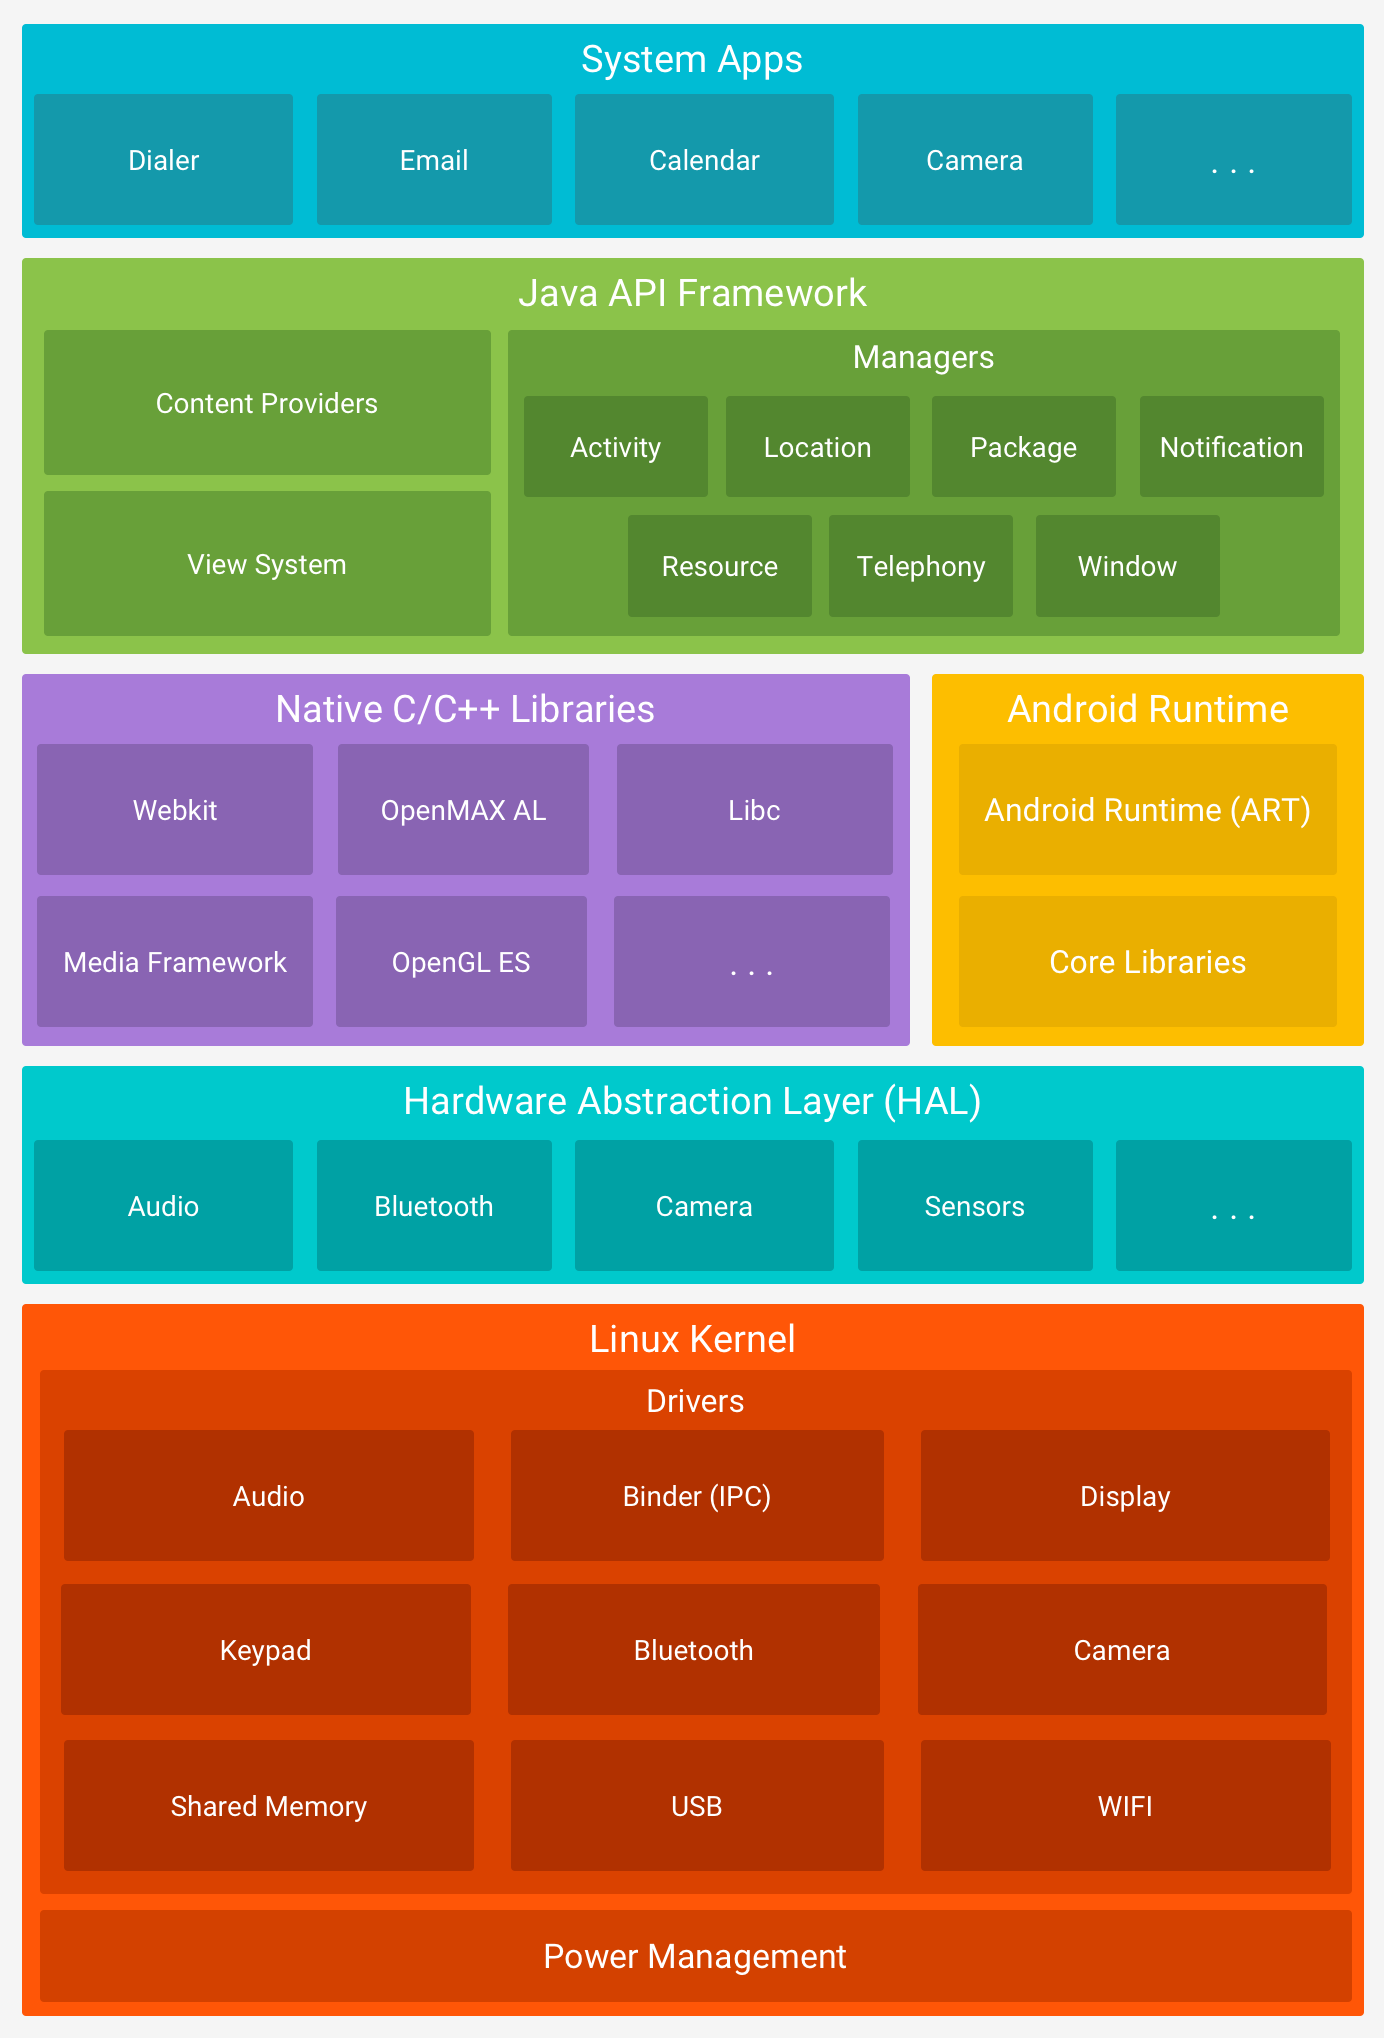
\includegraphics[height=200pt, keepaspectratio=true]{figuras/fundamentos/TheAndroidSoftwareStack.png}
        \caption{Esquema em blocos do SO do Android}
        \label{The Android software stack}
      \end{figure}
    \end{frame}

\end{document}


